\section{Installing Certificate Services}
\subsection{Activities}

\noindent {\bf{Bước 1:}} Truy cập vào đường dẫn \href{https://www.microsoft.com/en-us/evalcenter/evaluate-windows-server-2016}{Link} để download file ISO. Sau đó, chọn {\bf Download the ISO}.

\begin{figure}[!htb]
    \centering
    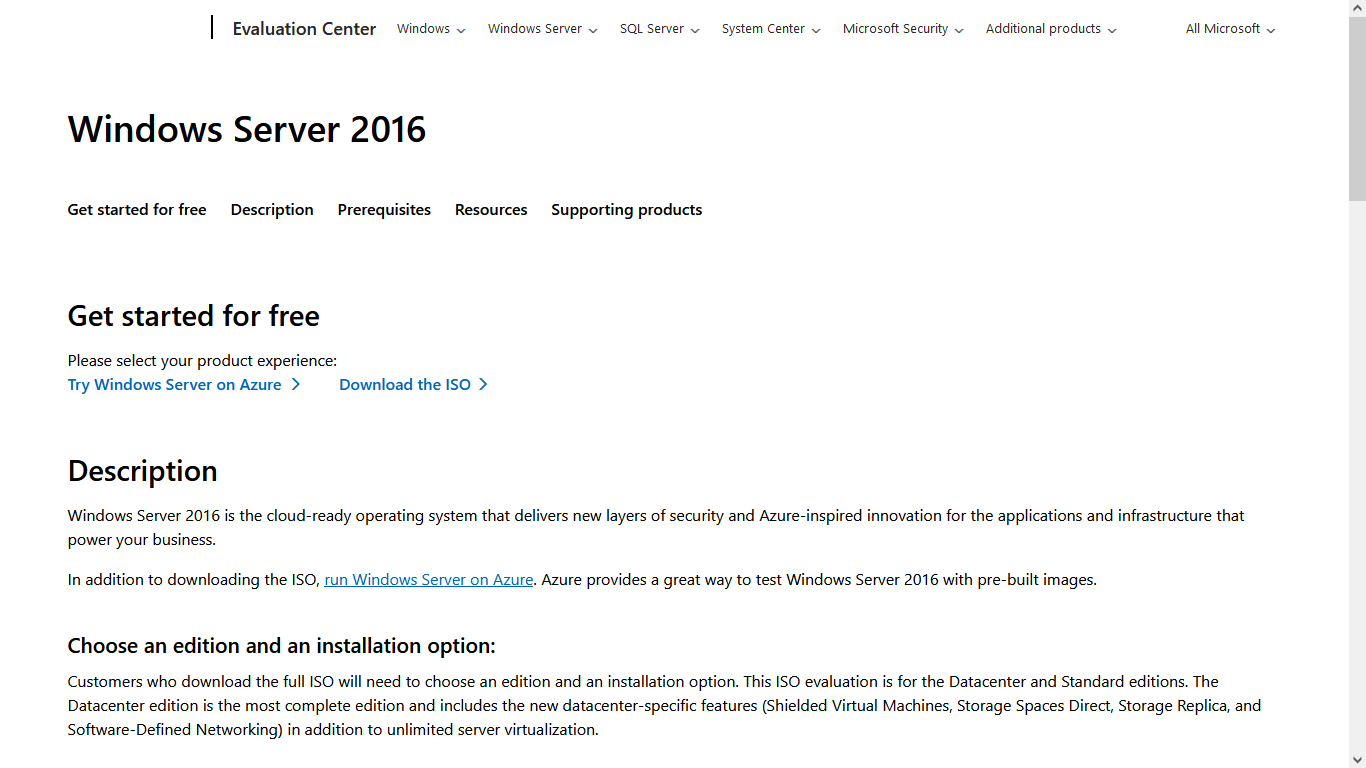
\includegraphics[width=1\linewidth]{figure//chapter4//lab4_1/download_iso.png}
    \caption{Màn hình tải file ISO}
    \label{fig:enter-label}
\end{figure}

\noindent {\bf{Bước 2:}} Điền các thông tin cần thiết rồi chọn {\bf Download}.

\begin{figure}[!htb]
    \centering
    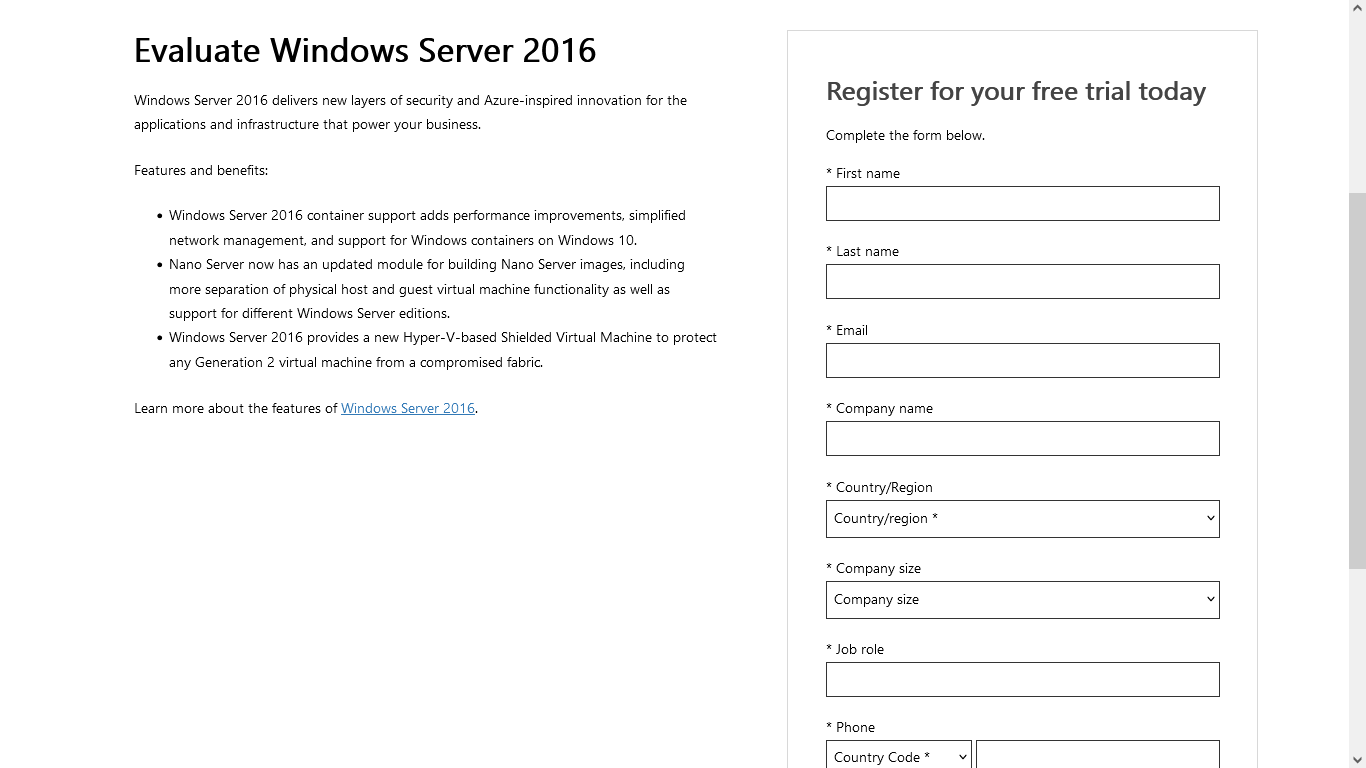
\includegraphics[width=1\linewidth]{figure//chapter4//lab4_1/input_info.png}
    \caption{Nhập thông tin cá nhân}
    \label{fig:enter-label}
\end{figure}

\noindent Sau đó chọn phiên bản phù hợp rồi lưu vào máy.

\vskip 0.5cm
\noindent {\bf{Bước 3:}} Tải VirtualBox và tạo ra một máy ảo Windows bằng file ISO vừa tải. Chọn Microsoft Windows và Windows 2016. Khởi động máy ảo.

\begin{figure}[!htb]
    \centering
    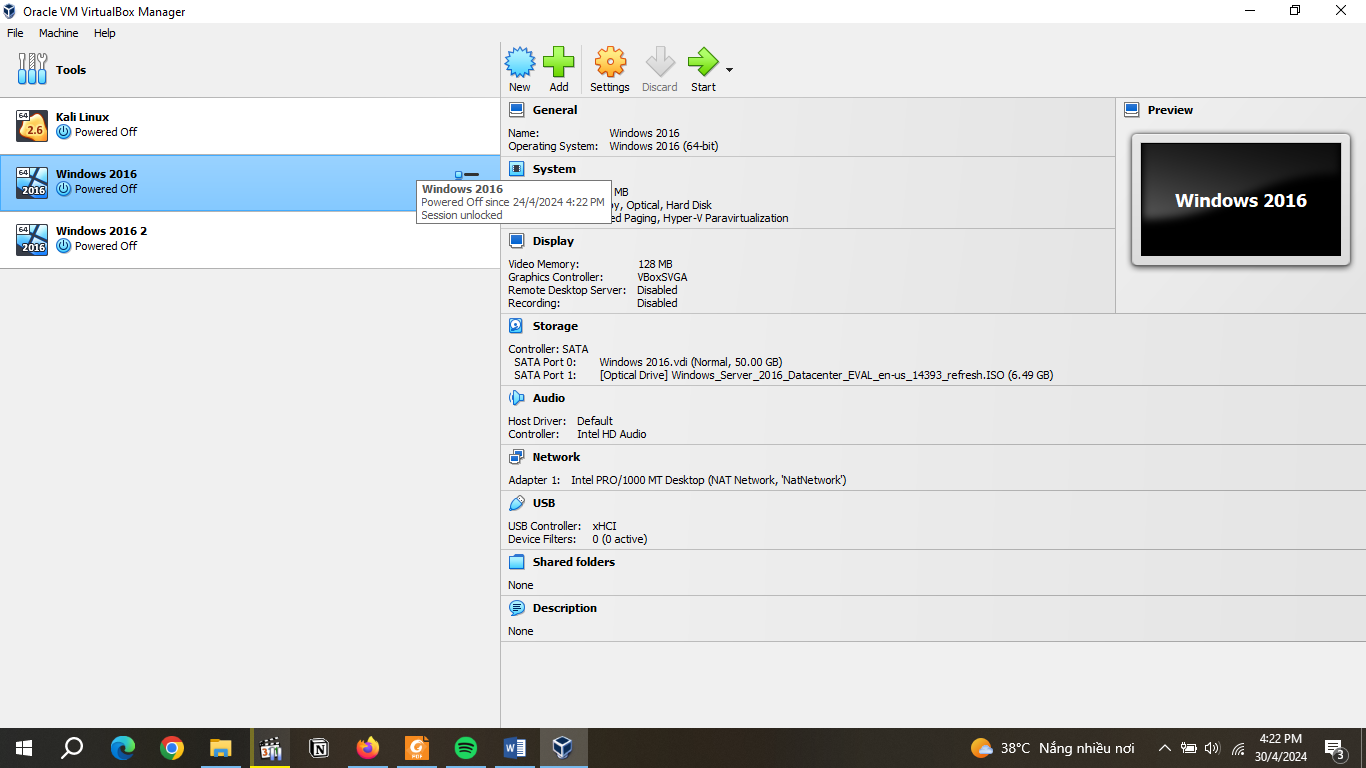
\includegraphics[width=1\linewidth]{figure//chapter4//lab4_1/start_vm.png}
    \caption{Khởi động máy ảo Windows 2016}
    \label{fig:enter-label}
\end{figure}

\vskip 0.5cm
\noindent {\bf{Bước 4:}} Chọn ngôn ngữ, thời gian và bàn phím phù hợp. Nhấn {\bf Install Now} để tiến hành cài đặt. Tại phần chọn Windows Setup, chọn {\bf Windows Server 2016 Standard Evaluation (Desktop Experience)}.

\begin{figure}[!htb]
    \centering
    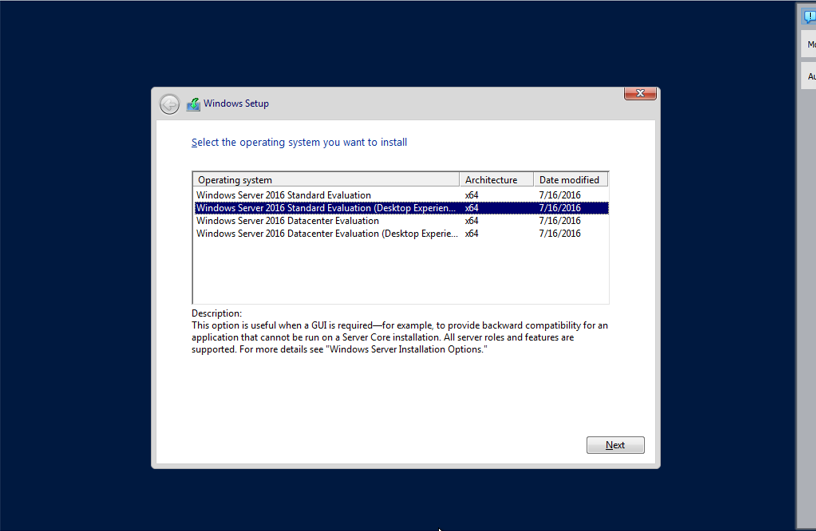
\includegraphics[width=0.8\linewidth]{figure//chapter4//lab4_1/select_os.png}
    \caption{Chọn hệ điều hành}
    \label{fig:enter-label}
\end{figure}

\vskip 0.5cm

\newpage

\noindent {\bf{Bước 5:}} Chọn {\bf Custom: Install Windows only (advanced)}. 

\begin{figure}[!htb]
    \centering
    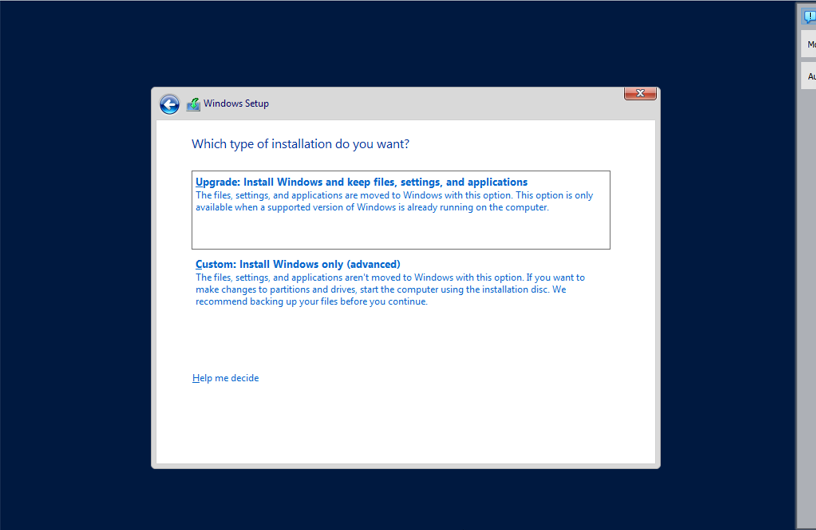
\includegraphics[width=1\linewidth]{figure//chapter4//lab4_1/select_setup_type.png}
    \caption{Chọn cách cài đặt}
    \label{fig:enter-label}
\end{figure}

\noindent {\bf{Bước 6:}} Tiếp tục chọn Next và cài đặt mật khẩu cho Administrator là {\bf Pa\$\$word}. Sau đó đăng nhập vào hệ thống với tài khoản Administrator.

\begin{figure}[!htb]
    \centering
    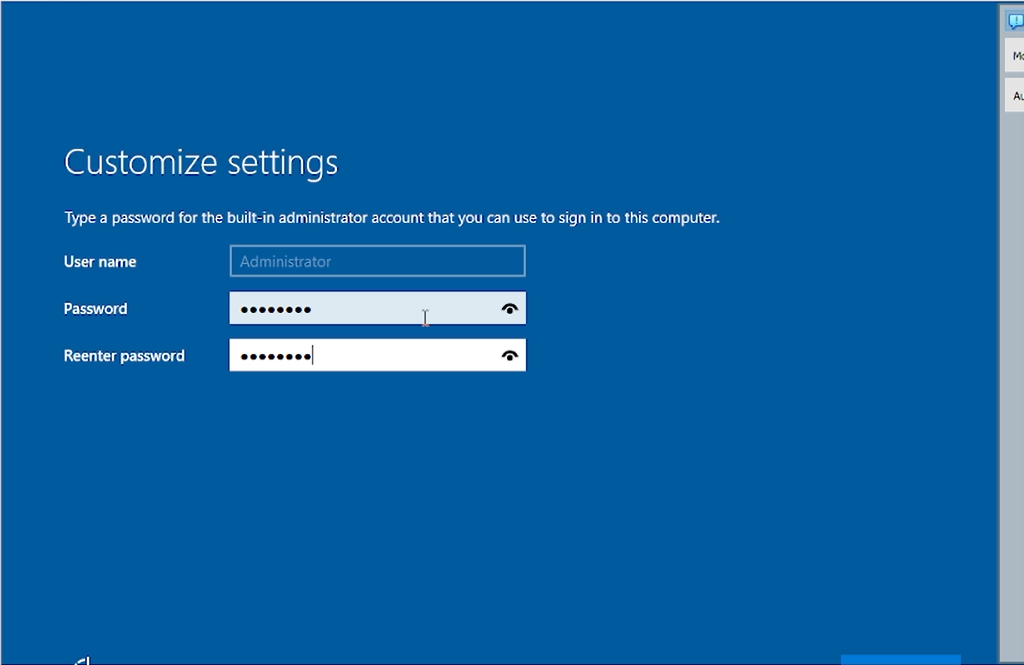
\includegraphics[width=1\linewidth]{figure//chapter4//lab4_1/enter_password.png}
    \caption{Enter Caption}
    \label{fig:enter-label}
\end{figure}

\noindent {\bf{Bước 7:}} Mở Server Manager, chọn \textbf{Manage} rồi chọn \textbf{Add Roles and Features}. Click \textbf{Next} cho tới khi thấy màn hình \textbf{Server Roles}.

\begin{figure}[!htb]
    \centering
    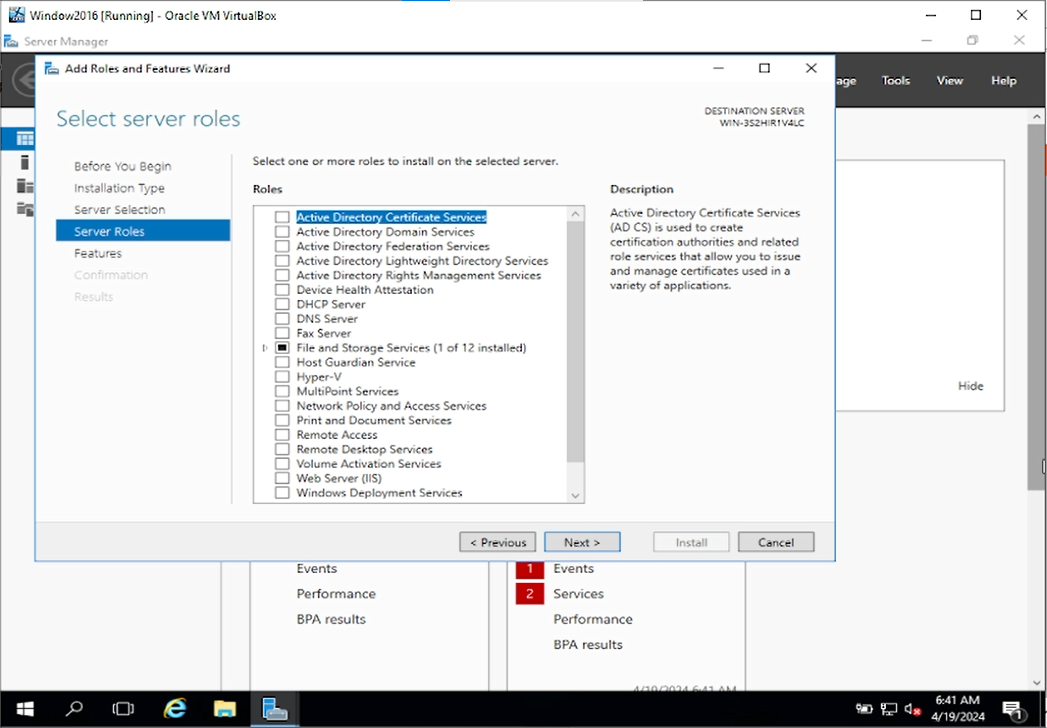
\includegraphics[width=0.9\linewidth]{figure//chapter4//lab4_1/select_add_roles_and_features.png}
    \caption{Màn hình Server Roles}
    \label{fig:enter-label}
\end{figure}

% \newpage

\noindent {\bf{Bước 8:}} Chọn \textbf{Active Directory Domain Services}. Sau đó chọn \textbf{Add Feature} ở màn hình hiện lên. Tiếp theo nhấn \textbf{Next} liên tục rồi \textbf{Install}.

\begin{figure}[!htb]
    \centering
    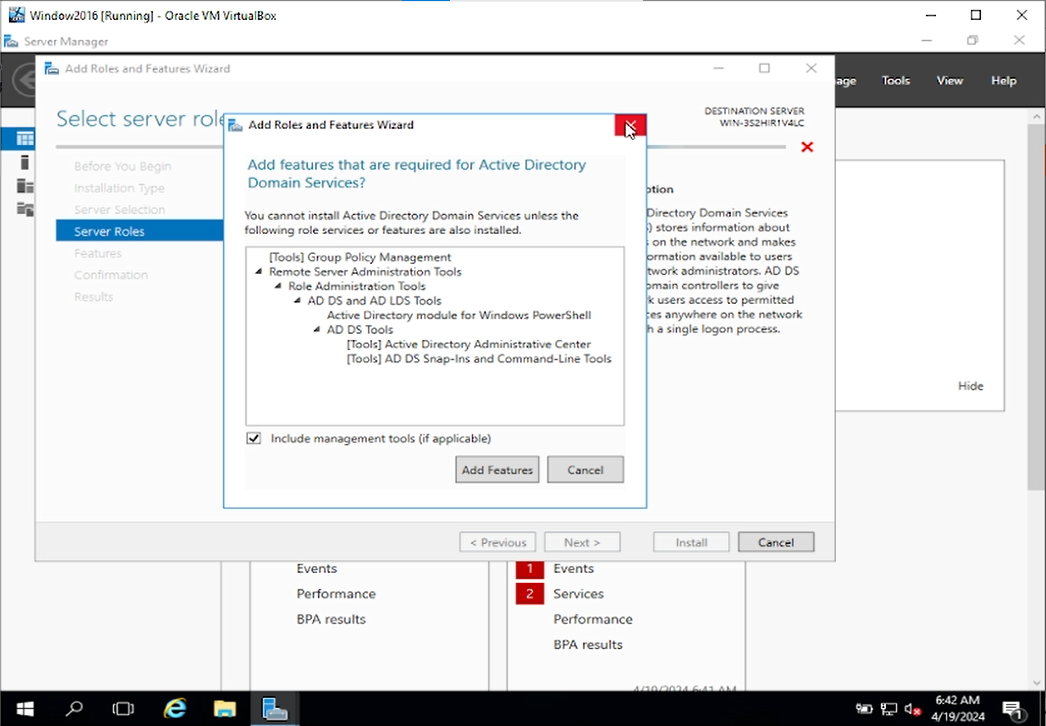
\includegraphics[width=0.9\linewidth]{figure//chapter4//lab4_1/add_feature.png}
    \caption{Màn hình Add Features}
    \label{fig:enter-label}
\end{figure}

\noindent {\bf{Bước 9:}} Chọn vào cờ thông báo ở phía trên màn hình và chọn \textbf{Promote this server to a domain controller}.

\begin{figure}[!htb]
    \centering
    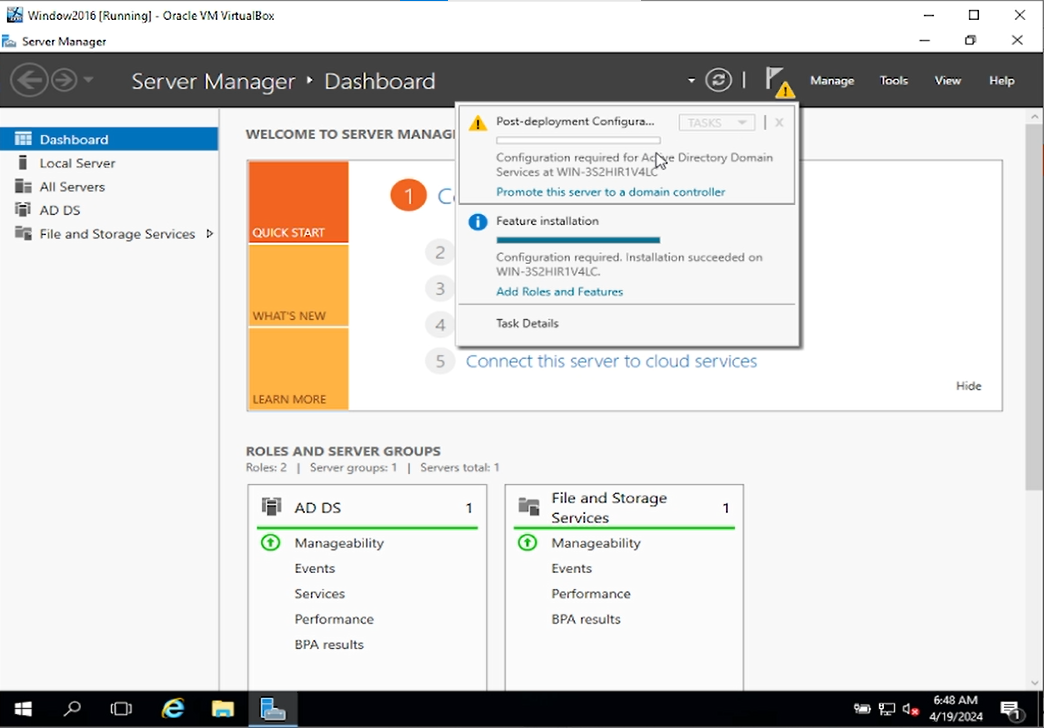
\includegraphics[width=0.9\linewidth]{figure//chapter4//lab4_1/promote_server.png}
    \caption{Chọn cờ thông báo}
    \label{fig:enter-label}
\end{figure}

\noindent {\bf{Bước 10:}} Chọn \textbf{Add a new forest} và điền \textbf{Test.local} vào phần \textbf{Root domain name}.

\begin{figure}[!htb]
    \centering
    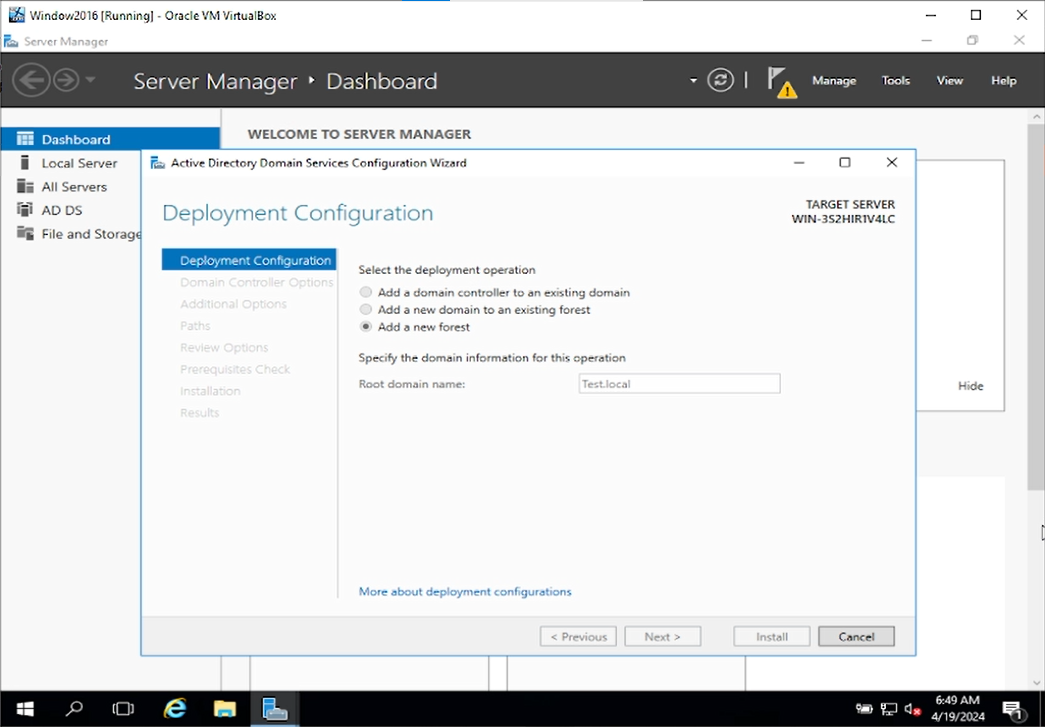
\includegraphics[width=0.9\linewidth]{figure//chapter4//lab4_1/test_local.png}
    \caption{Add a new forest}
    \label{fig:enter-label}
\end{figure}

\noindent {\bf{Bước 11:}} Điền mật khẩu là \textbf{Pa\$\$word}, rồi chọn \textbf{Next} hai lần.

\begin{figure}[!htb]
    \centering
    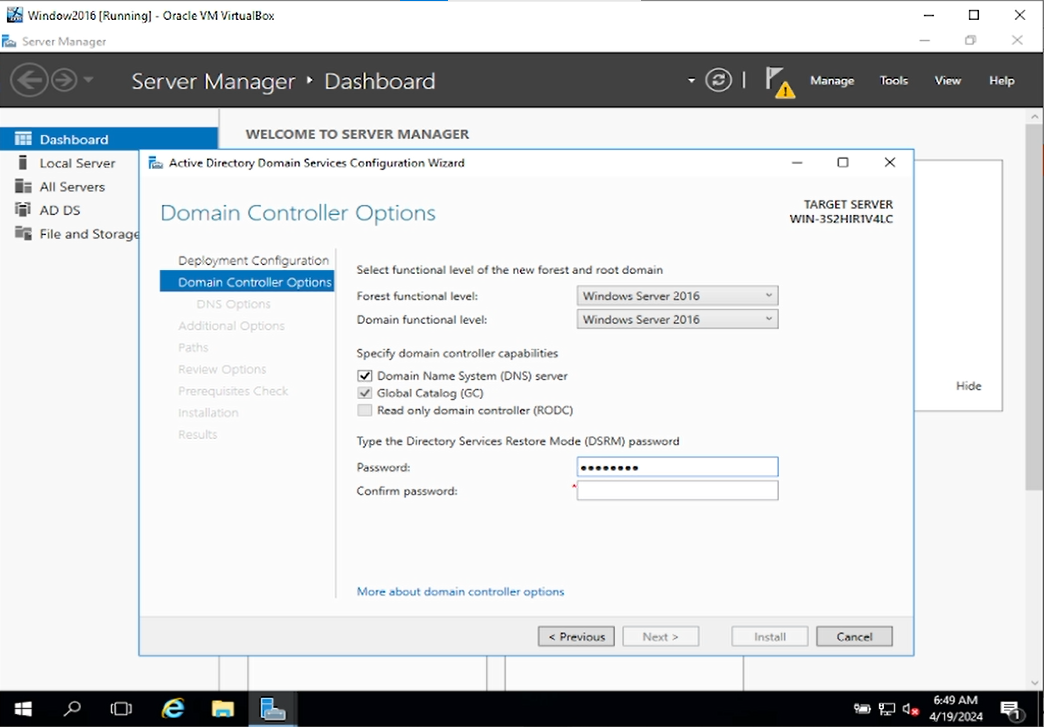
\includegraphics[width=0.9\linewidth]{figure//chapter4//lab4_1/enter_password_2.png}
    \caption{Nhập DSMR Password}
    \label{fig:enter-label}
\end{figure}

\noindent {\bf{Bước 11:}} Nhập \textbf{TEST} cho phần NetBIOS domain name và chọn \textbf{Next} ba lần.

\begin{figure}[!htb]
    \centering
    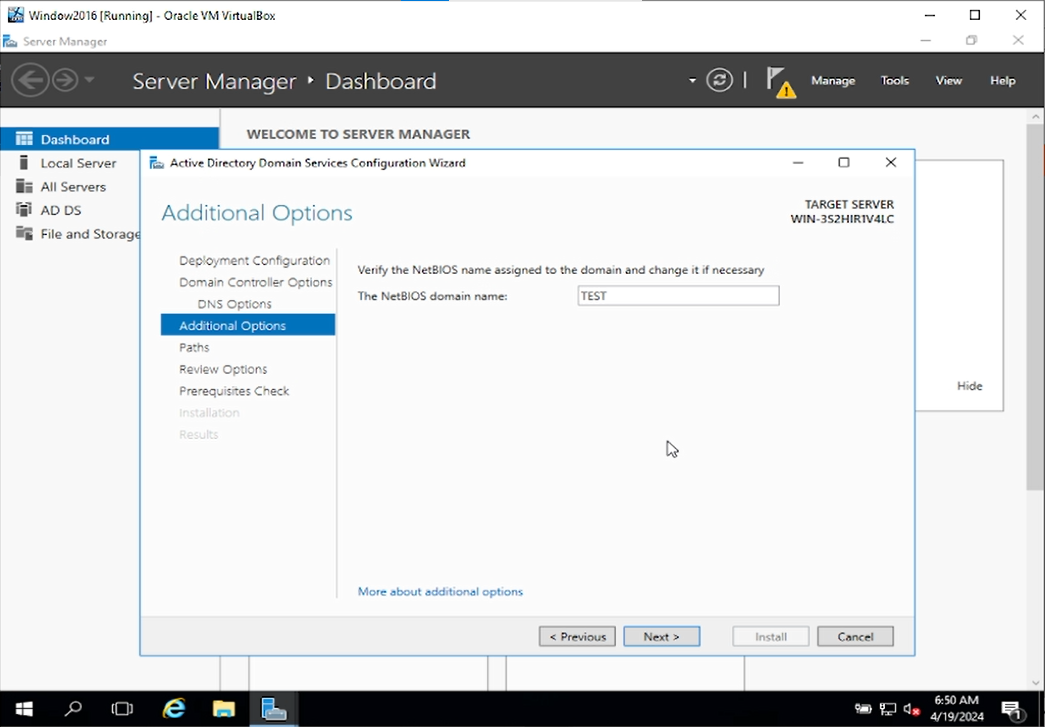
\includegraphics[width=0.9\linewidth]{figure//chapter4//lab4_1/enter_netbios_domain_name.png}
    \caption{Nhập NetBIOS domain name}
    \label{fig:enter-label}
\end{figure}

\noindent Tiếp tục chọn \textbf{Next} và cuối cùng chọn \textbf{Install}.

\noindent {\bf{Bước 12:}} Lặp lại quá trình cho tới khi gặp phải màn hình Server Roles. Tại đây, chọn \textbf{Active Directory Certificate Services}. Chọn \textbf{Add Features}.

\begin{figure}[!htb]
    \centering
    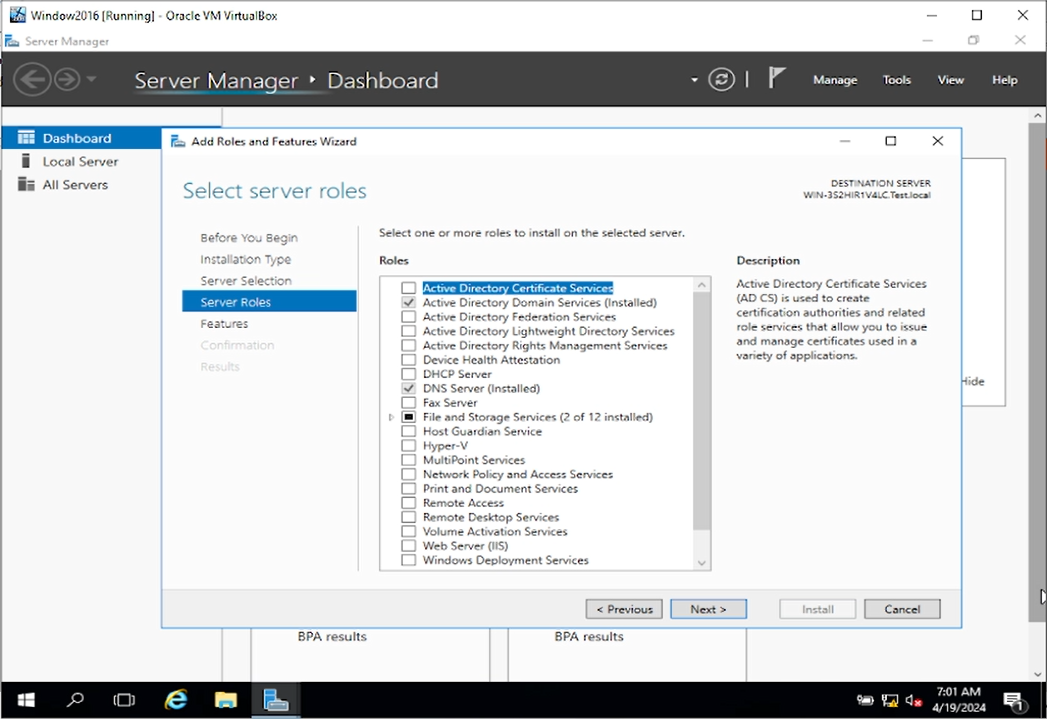
\includegraphics[width=0.9\linewidth]{figure//chapter4//lab4_1/add_active_domain_certificate_services.png}
    \caption{Chọn Active Directory Certificate Servicies}
    \label{fig:enter-label}
\end{figure}

\noindent {\bf{Bước 13:}} Cứ thế tiếp tục cho tới màn hình \textbf{AD CS} và\textbf{Role Services}. Chọn \textbf{Certification Authority} và \textbf{Certification Authority Web Enrollment}.

\begin{figure}[!htb]
    \centering
    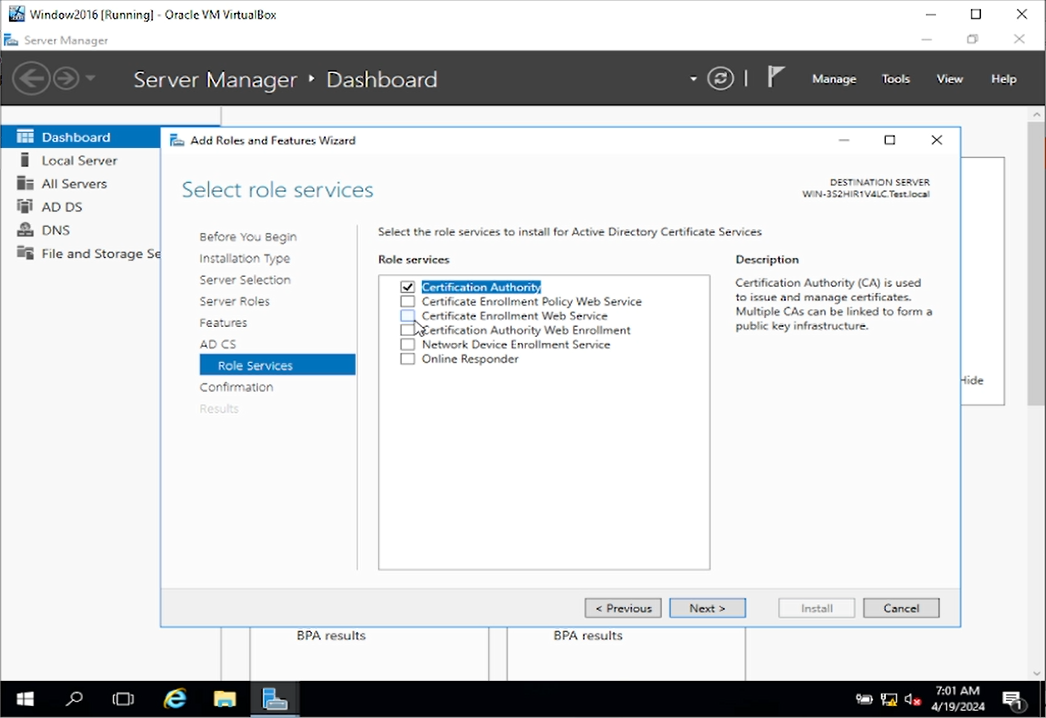
\includegraphics[width=0.9\linewidth]{figure//chapter4//lab4_1/role_service.png}
    \caption{Màn hình Role Services}
    \label{fig:enter-label}
\end{figure}

\noindent Chọn \textbf{Add Feature}, chọn \textbf{Next} và cuối cùng là \textbf{Install}.

\noindent {\bf{Bước 14:}} Vào cờ thông báo, chọn \textbf{Configure Active Directory Certificate Services on the destination server}. 

\begin{figure}[!htb]
    \centering
    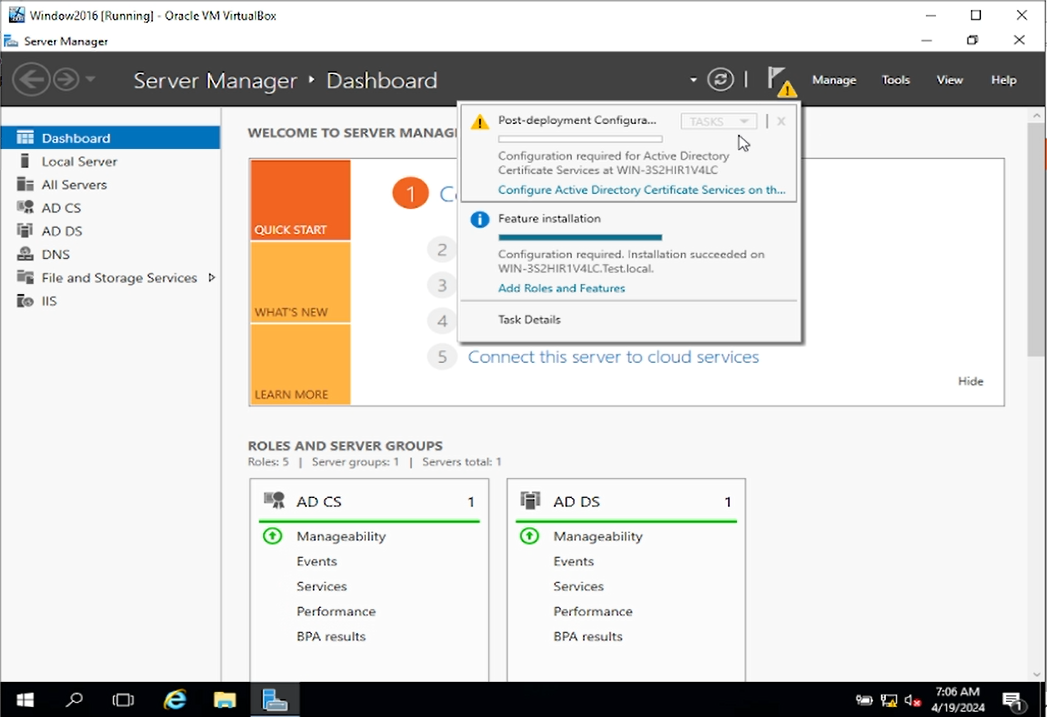
\includegraphics[width=0.9\linewidth]{figure//chapter4//lab4_1/configure_active_directory.png}
    \caption{Màn hình chọn cờ thông báo}
    \label{fig:enter-label}
\end{figure}

\noindent Chọn \textbf{Next} ở màn hình Credentials, chọn \textbf{Certification Authority} và \textbf{Certification Authority Web Enrollment}.

\begin{figure}[!htb]
    \centering
    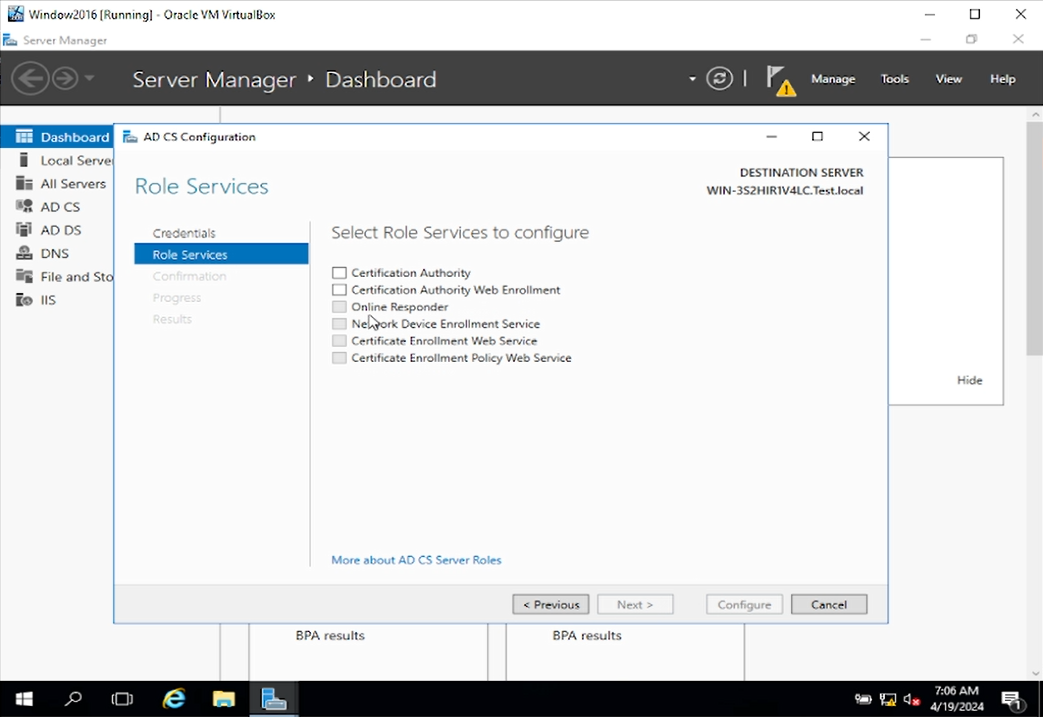
\includegraphics[width=0.85\linewidth]{figure//chapter4//lab4_1/configure_service.png}
    \caption{Chọn Service cần cấu hình}
    \label{fig:enter-label}
\end{figure}

\noindent {\bf{Bước 15:}} Trong các cửa sổ sau đó, sử dụng các lựa chọn đã được chọn mặc định và chọn \textbf{Next}. Cuối cùng chọn \textbf{Configure}.

\begin{figure}[!htb]
    \centering
    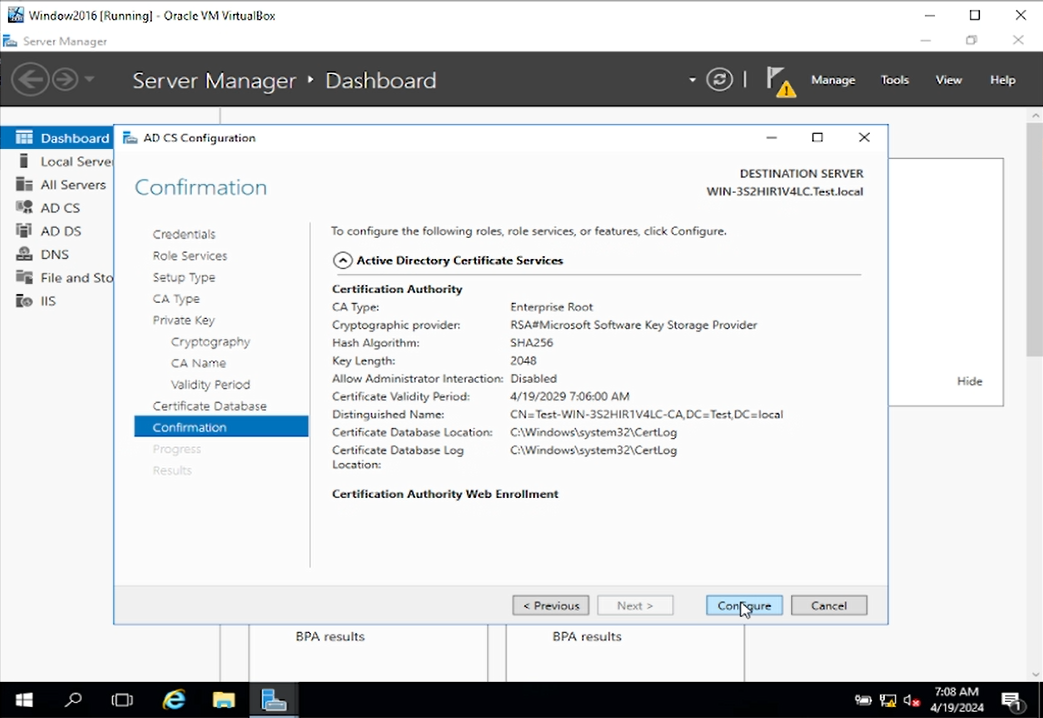
\includegraphics[width=0.9\linewidth]{figure//chapter4//lab4_1/configure_window.png}
    \caption{Màn hình cấu hình AD CS}
    \label{fig:enter-label}
\end{figure}

\noindent {\bf{Bước 16:}} Sau khi cài đặt xong, vào \textbf{Search Windows} và nhập mmc.

\begin{figure}[!htb]
    \centering
    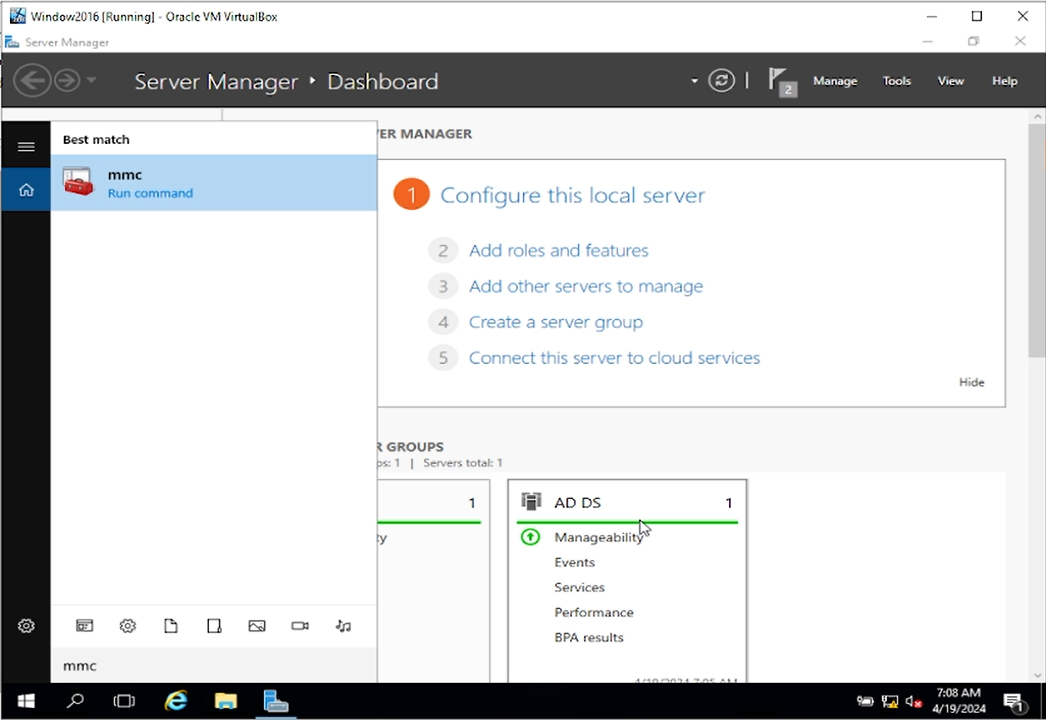
\includegraphics[width=0.9\linewidth]{figure//chapter4//lab4_1/mmc.png}
    \caption{Chọn mmc}
    \label{fig:enter-label}
\end{figure}

\newpage

\noindent {\bf{Bước 17:}} Chọn \textbf{File}, chọn \textbf{Add/Remove Snap-ins}. Sau đó, thêm \textbf{Add Certificate Templates}, \textbf{Certification Authority (Local), Enterprise PKI} và \textbf{Internet Information Service (IIS) Manager}.

\begin{figure}[!htb]
    \centering
    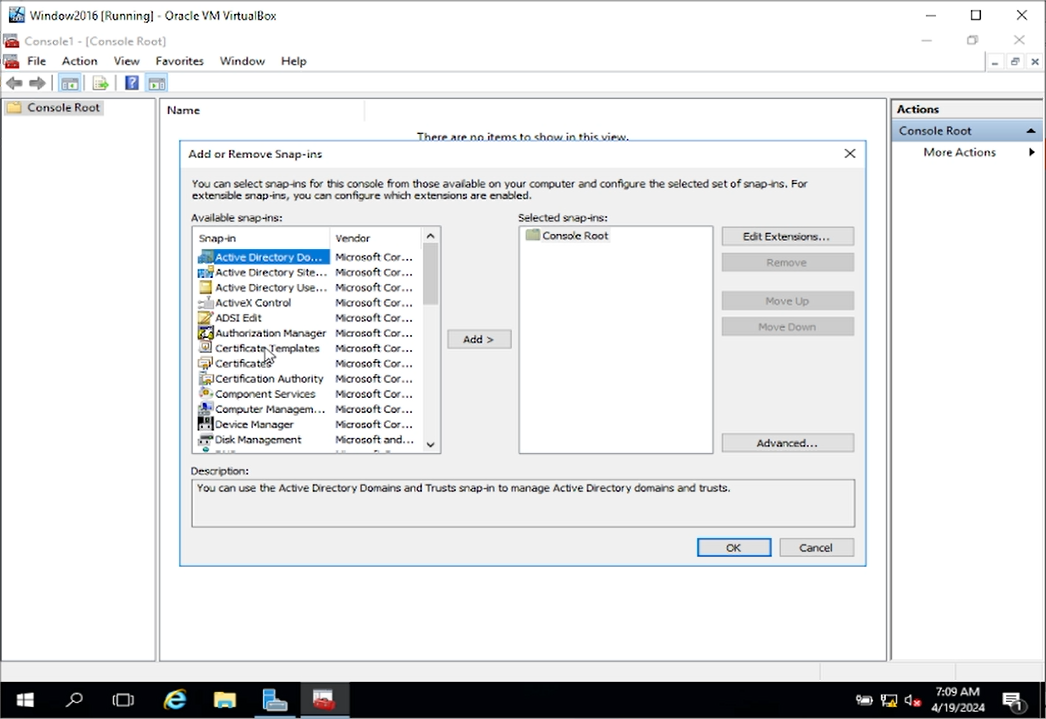
\includegraphics[width=0.9\linewidth]{figure//chapter4//lab4_1/add_snap_in.png}
    \caption{Thêm Snap-ins}
    \label{fig:enter-label}
\end{figure}

\noindent Kết quả nhận được như sau.

\begin{figure}[!htb]
    \centering
    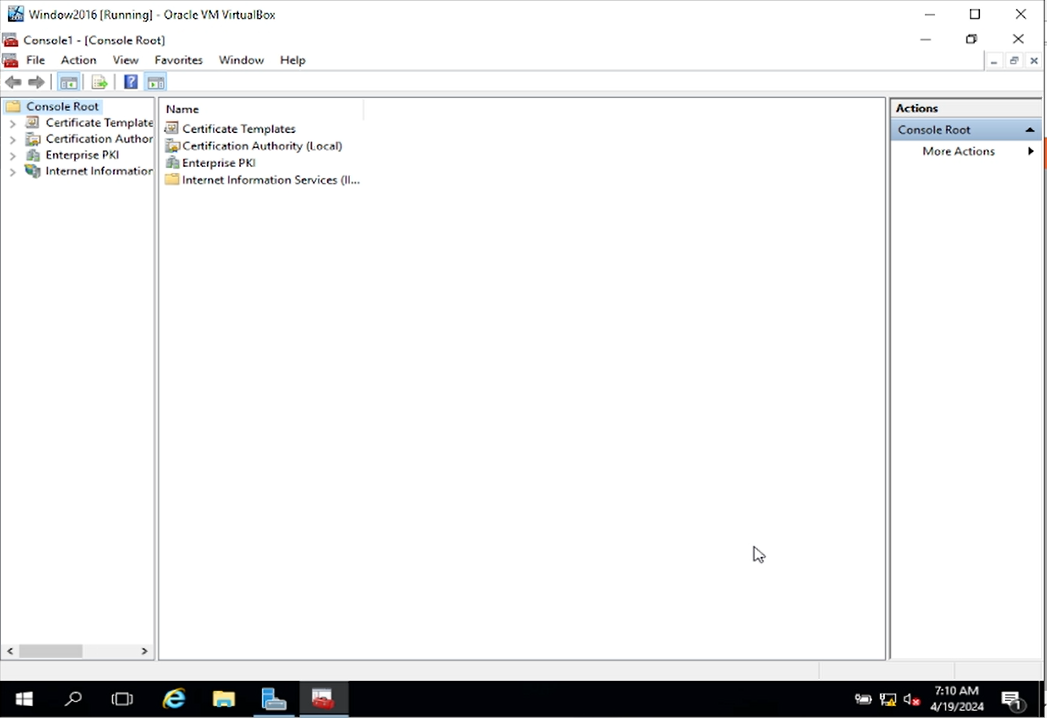
\includegraphics[width=0.9\linewidth]{figure//chapter4//lab4_1/result.png}
    \caption{Kết quả màn hình mmc}
    \label{fig:enter-label}
\end{figure}

\subsection{Review Questions}

\noindent \textbf{Câu 1:} 

B: Active Directory Domain Services.

\noindent \textbf{Câu 2:} 

B: Online Responder.

C: World Wide Web Publishing Service.

D: Network Device Enrollment Service.

\noindent \textbf{Câu 3:} 

C: Enhance certificate revocation checking by setting up an online responder.

\noindent \textbf{Câu 4:} True.

\noindent \textbf{Câu 5:} 


D: A stand-alone CA is integrated with Active Directory Domain Services.